%%\documentclass[referee,sn-basic]{sn-jnl}% referee option is meant for double line spacing

%%\documentclass[lineno,sn-basic]{sn-jnl}% Basic Springer Nature Reference Style/Chemistry Reference Style

%%\documentclass[pdflatex,sn-basic]{sn-jnl}% Basic Springer Nature Reference Style/Chemistry Reference Style

%%\documentclass[sn-basic]{sn-jnl}% Basic Springer Nature Reference Style/Chemistry Reference Style
%%\documentclass[sn-mathphys]{sn-jnl}% Math and Physical Sciences Reference Style

%%\documentclass[sn-aps]{sn-jnl}% American Physical Society (APS) Reference Style
\documentclass[sn-vancouver]{sn-jnl}% Vancouver Reference Style
%%\documentclass[sn-apa]{sn-jnl}% APA Reference Style
%%\documentclass[sn-chicago]{sn-jnl}% Chicago-based Humanities Reference Style
%%\documentclass[sn-standardnature]{sn-jnl}% Standard Nature Portfolio Reference Style
%%\documentclass[default]{sn-jnl}% Default
%%\documentclass[default,iicol]{sn-jnl}% Default with double column layout

\usepackage{bbding}
\usepackage{caption}
\graphicspath{ {C:/Users/sofya/Desktop/PC/pdf_figures/} }

\jyear{2021}%

%% as per the requirement new theorem styles can be included as shown below
\theoremstyle{thmstyleone}%
\newtheorem{theorem}{Theorem}%  meant for continuous numbers
%%\newtheorem{theorem}{Theorem}[section]% meant for sectionwise numbers
%% optional argument [theorem] produces theorem numbering sequence instead of independent numbers for Proposition
\newtheorem{proposition}[theorem]{Proposition}% 
%%\newtheorem{proposition}{Proposition}% to get separate numbers for theorem and proposition etc.

\theoremstyle{thmstyletwo}%
\newtheorem{example}{Example}%
\newtheorem{remark}{Remark}%

\theoremstyle{thmstylethree}%
\newtheorem{definition}{Definition}%

\raggedbottom
%%\unnumbered% uncomment this for unnumbered level heads

\begin{document}

\title[Analysis of Fairness Measures]{Analysis of Fairness Measures}

%%=============================================================%%
%% Prefix	-> \pfx{Dr}
%% GivenName	-> \fnm{Joergen W.}
%% Particle	-> \spfx{van der} -> surname prefix
%% FamilyName	-> \sur{Ploeg}
%% Suffix	-> \sfx{IV}
%% NatureName	-> \tanm{Poet Laureate} -> Title after name
%% Degrees	-> \dgr{MSc, PhD}
%% \author*[1,2]{\pfx{Dr} \fnm{Joergen W.} \spfx{van der} \sur{Ploeg} \sfx{IV} \tanm{Poet Laureate} 
%%                 \dgr{MSc, PhD}}\email{iauthor@gmail.com}
%%=============================================================%%

\author*[]{\fnm{Sofya} \sur{Aksenyuk}}

\author[]{\fnm{Uladzimir} \sur{Ivashka}}

\author[]{\fnm{Oleksandr} \sur{Yasinskyi}}

\maketitle

\section{Introduction}\label{sec1}

Artificial Intelligence (AI) has become an integral part of our world today, and the field of Computer Science is no exception.

Machine Learning (ML), a subset of AI, is widely used as one of its scientific methods. It focuses on analyzing and interpreting data patterns and structures to facilitate learning, reasoning, and decision-making without the need for direct human interaction. In simpler terms, machine learning enables users to input data into a computer algorithm, which then analyzes the data to further render recommendations and decisions based solely on what was given. If any corrections are found, the algorithm can use that knowledge to make better decisions in the future.

ML can be found in a variety of fields in our daily lives. Its value has already been recognized by all major industries that deal with large amounts of data. It provides access to a wide range of useful methods that can aid in expanding a business into different domains by gaining useful insights from the data. 

However, ML is not just about running businesses. Data can also be processed or learned from in an incorrect manner, resulting in a lack of objectivity in decision-making. The topic of discrimination affects all of us to some extent. There are numerous examples of employers being unfair in their hiring practices or different payments based on personal traits. This is where the idea of the analysis comes in - to examine fairness using AI.

Fairness in general refers to the absence of prejudice or bias towards a group of people or an individual based on certain characteristics, the quality of treating people equally or in a way that is right or reasonable. AI decision systems are widely used nowadays, meaning that it has a significant impact on others' lives. Therefore, it is essential to ensure that discriminatory decisions do not take place, meaning that it does not take into account one's race, age, gender, or any other personal trait.

To achieve this, several challenges must be encountered, such as dealing with imbalanced data, determining the appropriate way of measuring fairness, and determining which metric to use for that purpose. Therefore, in this analysis, we focus on determining the most appropriate measures for calculating fairness and the conditions for that. 

Our research task is to answer how different types of data bias settings affect the performance of fairness measures. Specifically, it concerns examining the susceptibility of these measures to various scenarios of data imbalance, such as skewed class proportions or class imbalance.

\section{Related works}\label{sec2}

Fairness measures have been extensively reviewed in recent years [1,3,4,5,6], supported by some earlier works [2,7]. However, the aforementioned studies are mainly based on the evaluation of classifiers and their general practical applications. Additionally, these works perform tests on particular datasets, which makes them dataset-dependent. 

Therefore, it is crucial for us to study fairness measures on a general dataset, which makes it possible to examine the properties of the measures in diverse settings, such as different levels of class imbalance or representation and feature biases. 

By having results of overall fairness measures behavior, regardless of a dataset, it will be possible to define the best measure when it comes to calculating fairness and to answer the question of whether we are fair in general.

\section{Methodology}\label{sec3}

\subsection{The impact of imbalance data}\label{subsec1}

The study focuses on the concept of privileged (majority) and unprivileged (minority) groups. To further illustrate the concept of unbalanced data, consider a hypothetical example of a classification task where the goal is to identify a rare disease in patients. Due to the rarity of the disease, only 5\% of the samples in the training set have the disease. In this scenario, a classifier that assumes all samples are healthy would achieve high accuracy but would not effectively perform the task of identifying the rare disease. To address this issue, various methods have been developed to mitigate the negative impact of class imbalance.

We can talk about unbalanced data when the classes in the problem are not similar numerously represented. This can occur for two or more classes, but in this paper, we will focus on binary classification. When there are only two classes, the more numerous class is referred as the majority class, and the less numerous class is referred as the minority class. The degree of imbalance can be quantified by calculating the Imbalance Ratio (IR), also known as minority ratio in some researches. The most commonly used formula for calculating:

\begin{equation}
IR = N_{mj} / N_{mn}\label{eq1}
\end{equation}

where $N_{mj}$ is the size of the majority class, and $N_{mn}$ is the size of the minority class. This formula calculates how many times the majority class is larger than the minority class.

Another measure related to Imbalance Ratio is Group Ratio (GR). While Imbalance Ratio quantifies class imbalance, Group Ratio measures the imbalance of groups distinguished by a sensitive attribute. The formula for Group Ratio is:

\begin{equation}
GR = N_{mn}  / (N_{mn} + N_{mj}) \label{eq2}
\end{equation}

where $N_{mn}$ is the size of the minority group and $N_{mj}$ is the size of the majority group. It is should be mentioned that the determination of which group constitutes the minority is a matter of convention and not based on a fixed numerical threshold. The minority group can range from as low as 1\% to as high as 50\%.

\subsection{Dataset generation}\label{subsec2}

In light of previous considerations, our study chooses to focus on several fairness measures that center around prediction probabilities represented by confusion matrices, e.g., statistical parity, equal opportunity, etc.

A confusion matrix, also known as an error matrix, is a table that is commonly used to evaluate the performance of a binary or multiclass classifier. The columns of the matrix represent the predicted classes, while the rows represent the actual classes. The diagonal elements of the matrix represent the number of correct predictions made by the classifier, also known as true positives (TP) and true negatives (TN). The off-diagonal elements of the matrix represent the number of incorrect predictions made by the classifier, also known as false positives (FP) and false negatives (FN). In addition to providing a summary of the classifier's performance, the confusion matrix can also be used to calculate various performance metrics, what we used in our work. 

Group fairness measures can be defined on subsets of confusion matrices. However, the concept of sensitive groups in fairness measures requires an examination of distributions within pairs of sum-constrained confusion matrices rather than a single confusion matrix. The objective of our study is to investigate how changes in the distributions of classes (regardless of a specific dataset) impact the values of fairness measures. Such an analysis will provide insight into which fairness measures are robust to class and group imbalance. This will allow the creation of guidelines for selecting appropriate fairness measures for a given scenario. Additionally, the study explores other forms of uneven data distributions, such as stereotypical bias. The term stereotypical bias refers to situations where sensitive groups are underrepresented within specific classes, despite being evenly distributed in the entire dataset.

At this stage of the study, it was necessary to find a dataset on which the previously selected fairness measures could be calculated. As far as we aim to analyze fairness measures across all levels of class and group imbalance independently of a specific data, the dataset has to contain all possible outcomes. In order to visualize the values of the measures as a function of changing Imbalance Ratio (IR) and Group Ratio (GR), we needed the dataset with the largest size n possible. For example, let n = 10, so we have a dataset of 10 individuals. Among them, there are majority class (denoted as i) and minority class (denoted as j) which are classified with a positive or negative result. 

Table 1 shows several rows, representing different versions of the combinations of confusions matrices that may exist for this problem. The generated dataset was loaded into the dataframe structure. For each version of the confusion matrix in the dataframe, IR, GR and all previously selected fairness measures were calculated. The dataframe was then filtered to obtain specific IR and GR combinations, and grouped to create histograms.

\begin{table}[h]
\begin{center}
\begin{minipage}{225pt}
\caption{Dataset snippet}\label{tab1}%
\begin{tabular}{|c|c|c|c|c|c|c|c|c|}
\hline
    & TP$_{i}$ & FP$_{i}$ & TN$_{i}$ & FN$_{i}$ & TP$_{j}$ & FP$_{j}$ & TN$_{j}$ & FN$_{j}$ \\ \hline
1   & 55    & 1     & 0     & 0     & 0     & 0     & 0     & 0     \\ \hline
2   & 55    & 0     & 1     & 0     & 0     & 0     & 0     & 0     \\ \hline
3   & 55    & 0     & 0     & 1     & 0     & 0     & 0     & 0     \\ \hline
4   & 55    & 0     & 0     & 0     & 1     & 0     & 0     & 0     \\ \hline
... & ...   & ...   & ...   & ...   & ...   & ...   & ...   & ...   \\ \hline
\end{tabular}
\end{minipage}
\end{center}
\end{table}

\subsection{Metrics}\label{subsec3}

In the realm of measures, there exist two distinct categories: difference and ratio. For the purpose of achieving perfect fairness, difference measures aim for a value of zero, while ratio measures aim for a value of one. In this study, our focus was solely on difference measures and as a result, we did not delve into the analysis of ratio measures.

\textbf{Accuracy Equality}:

\begin{equation}
\frac{TP_{j} + TN_{j}}{TP_{j} + TN_{j} + FP_{j} + FN_{j}} = \frac{TP_{i} + TN_{i}}{TP_{i} + TN_{i} + FP_{i} + FN_{i}} \label{eq3}
\end{equation}

Accuracy Equality Difference (AED) is a fairness metric that measures the difference in accuracy between different groups defined by a sensitive attribute, such as race or gender. AED can be calculated as the absolute difference in accuracy between the privileged group and the unprivileged group.

\textbf{Statistical Parity}:

\begin{equation}
\frac{TP_{j} + FP_{j}}{TP_{j} + TN_{j} + FP_{j} + FN_{j}} = \frac{TP_{i} + FP_{i}}{TP_{i} + TN_{i} + FP_{i} + FN_{i}} \label{eq4}
\end{equation}

Statistical Parity (SP) is a group fairness metric that compares the proportion of positive outcomes for different groups. SP can be calculated as the difference in the proportion of positive outcomes between the privileged group and the unprivileged group.

\textbf{Equal Opportunity}:

\begin{equation}
TPR_{j} = TPR_{i} \label{eq5}
\end{equation}

where,

\begin{equation}
TPR = \frac{TP}{TP + FN} \label{eq6}
\end{equation}

Equal Opportunity Difference (EOD) is a group fairness metric that compares the true positive rate (TPR) between different groups. EOD can be calculated as the absolute difference in the TPR between the privileged group and the unprivileged group.

\textbf{Predictive Equality}:

\begin{equation}
FPR_{j} = FPR_{i} \label{eq7}
\end{equation}

where,

\begin{equation}
FPR = \frac{FP}{FP + TN} \label{eq8}
\end{equation}

Predictive Equality Difference (PED) is a group fairness metric that compares the false positive rate (FPR) between different groups. PED can be calculated as the absolute difference in the FPR between the privileged group and the unprivileged group.

\textbf{Positive Predictive Parity}:

\begin{equation}
PPV_{j} = PPV_{i} \label{eq9}
\end{equation}

where,

\begin{equation}
PPV = \frac{TP}{FP + TP} \label{eq10}
\end{equation}

Positive Predictive Parity Difference (PPPD) is a group fairness metric that compares the positive predictive value (PPV) between different groups. PPPD can be calculated as the absolute difference in the PPV between the privileged group and the unprivileged group.

\textbf{Negative Predictive Parity}:

\begin{equation}
NPV_{j} = NPV_{i} \label{eq11}
\end{equation}

where,

\begin{equation}
NPV = \frac{TN}{FN + TN} \label{eq12}
\end{equation}

Negative Predictive Parity Difference (NPPD) is a group fairness metric that compares the negative predictive value (NPV) between different groups. NPPD can be calculated as the absolute difference in the NPV between the privileged group and the unprivileged group.

All of these metrics are useful in different contexts and use cases, and it's important to discover which ones are most appropriate for a particular situation. 

\subsection{Results}\label{subsec4}

\subsubsection{Properties}\label{subsubsec1}

For the purposes of analysis, a set of GR and IR values were selected: {0.25, 0.5, 0.75}, and the chosen metrics' distributions were plotted in relation to them. Additionally, the proportions of perfect fairness of the measures were analyzed depending on the IR values.

In the metric plots, the IR values are represented in columns, while the GR values are represented in rows. The x-axis represents the range of metric values from [-1, 1]. The y-axis, although on the same scale, represents the initial values divided by the total sum of counts, and can be interpreted as the probability of getting such values.

A large number of plots were obtained and are available [8].

\begin{table}[h]
\begin{center}
\begin{minipage}{300pt}
\caption{Table of Metric Properties. Properties can be found on plots in: [TPR] - symmetry around 0. [NaN] - red bar to the left. [Sh] - change in shape with increase in GR. [HP] - the highest value on y-axis. [PF] - spikes around 1.0 value on y-axis. [EP] - change in shape with increase in IR. [IJ] - value on y-axis on IR = 0.5.}\label{tab2}%
\resizebox{\columnwidth}{!}{%
\begin{tabular}{|c|l|cccc|c|c|}
\hline
\multicolumn{1}{|l|}{Symbol} &
  \multicolumn{1}{c|}{Property} &
  \multicolumn{1}{c|}{EOD} &
  \multicolumn{1}{c|}{PED} &
  \multicolumn{1}{c|}{PPPD} &
  NPPD &
  AED &
  SP \\ \hline
{[}TPR{]} &
  \multicolumn{1}{c|}{TPR$_{i}$ = TPR$_{j}$} &
  \multicolumn{1}{c|}{\Checkmark} &
  \multicolumn{1}{c|}{\Checkmark} &
  \multicolumn{1}{c|}{\Checkmark} &
  \Checkmark &
   &
   \\ \hline
{[}NaN{]} &
  \multicolumn{1}{c|}{Undefined numbers} &
  \multicolumn{1}{c|}{\Checkmark} &
  \multicolumn{1}{c|}{\Checkmark} &
  \multicolumn{1}{c|}{\Checkmark} &
  \Checkmark &
   &
   \\ \hline
{[}Sh{]} &
  \begin{tabular}[c]{@{}l@{}}Is it equally probable\\ to be fair with change\\ in GR\end{tabular} &
  \multicolumn{1}{c|}{\Checkmark} &
  \multicolumn{1}{c|}{\Checkmark} &
  \multicolumn{1}{c|}{} &
  \multicolumn{1}{c|}{} &
  \multicolumn{1}{c|}{\Checkmark} &
  \Checkmark \\ \hline
{[}HP{]} &
  \begin{tabular}[c]{@{}l@{}}Highest probability\\ of fairness obtained\end{tabular} &
  \multicolumn{4}{c|}{$\approx$ 0.9} &
  $\approx$ 0.8 &
  $\approx$ 0.05 \\ \hline
{[}PF{]} &
  \begin{tabular}[c]{@{}l@{}}Possibility of being\\ perfectly fair\end{tabular} &
  \multicolumn{4}{c|}{\Checkmark} &
  \Checkmark &
  \multicolumn{1}{l|}{} \\ \hline
{[}EP{]} &
  \begin{tabular}[c]{@{}l@{}}Is it equally probable\\ to be fair, regardless\\ of IR value\end{tabular} &
  \multicolumn{4}{l|}{} &
  \multicolumn{1}{l|}{} &
  \Checkmark \\ \hline
{[}IJ{]} &
  \begin{tabular}[c]{@{}l@{}}Probability of fairness\\ having $N_{i} = N_{j}$\end{tabular} &
  \multicolumn{4}{c|}{\textgreater{} 0.05} &
  \multicolumn{1}{l|}{$\approx$ 0.65} &
  \multicolumn{1}{l|}{$\approx$ 0.05} \\ \hline
\end{tabular}%
}
\end{minipage}
\end{center}
\end{table}

The PPPD metric, as demonstrated in Figure 2, provides interesting observations about the properties of Table ~\ref{tab2}. One notable feature is the symmetry of the [TPR] table property around the value of 0 in each subplot. However, it is important to note that NaN-values are present to the left of each subplot. The only subplots that exhibit symmetric distributions are those with IR or GR values of 0.5. This suggests that the probability of fairness changes as the proportion of minority group in the dataset increases.

When examining the [HP] property, the maximum value of chance to be fair is around 70\%. This can be observed in the subplot with IR = GR = 0.5. However, when looking at the [HP] property in relation to IR in Figure ~\ref{fig2} (PPF), the highest probability obtained is 0.9. The rest of the properties can also be found in Figure 3, including the [PF] property with a highest probability value close to perfect fairness (1.0) and the [EP] property, which was not detected in the PPPD metric, due to the drastic changes in the y-axis values from [-1, 1]. The [IJ] property is only equal to 0.05, indicating that there is only a 5\% level of fairness when the proportion of majority and minority groups in the dataset is equal.

\begin{figure}[h]%
\centering
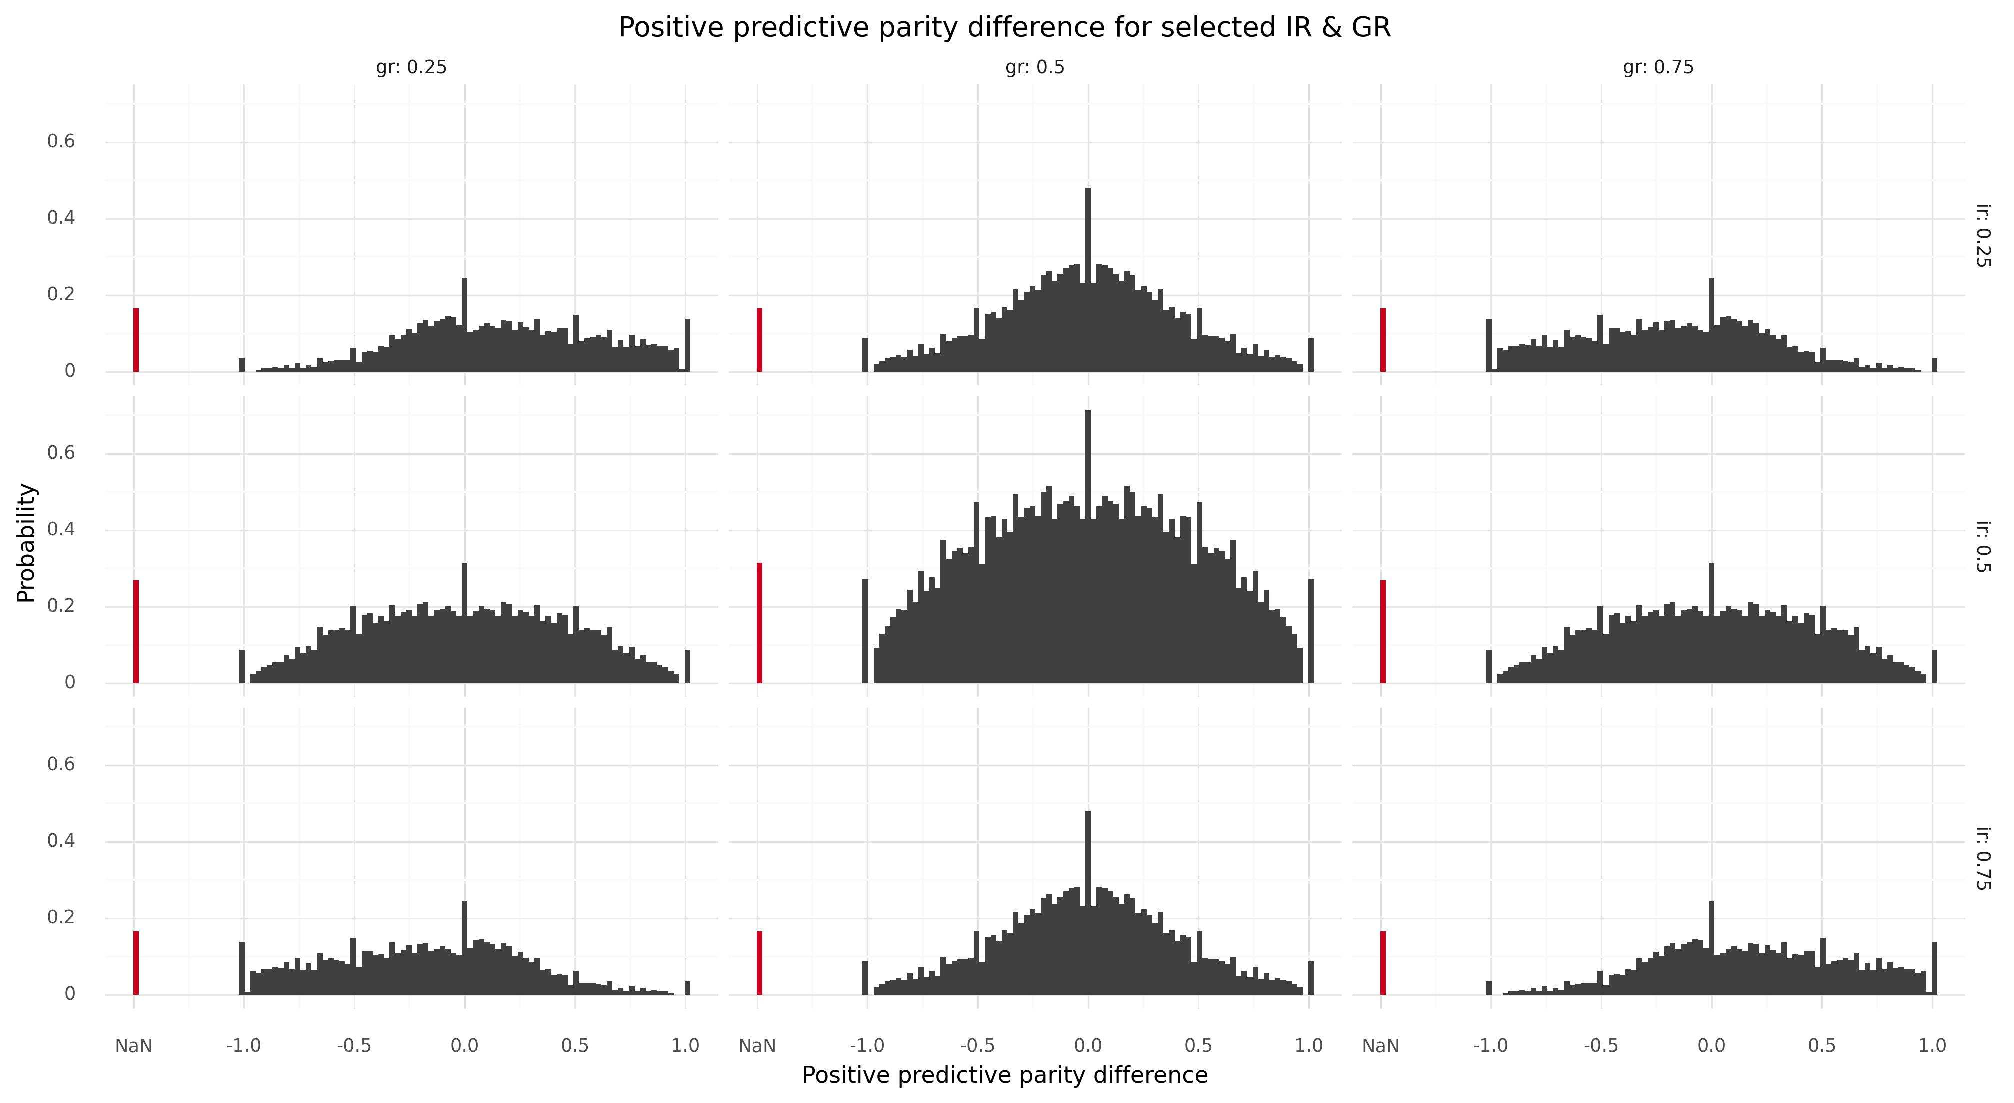
\includegraphics[width=0.9\textwidth]{PPPD}
\caption{Positive Predictive Parity Difference Plot}\label{fig1}
\end{figure}

\begin{figure}[h]%
\centering
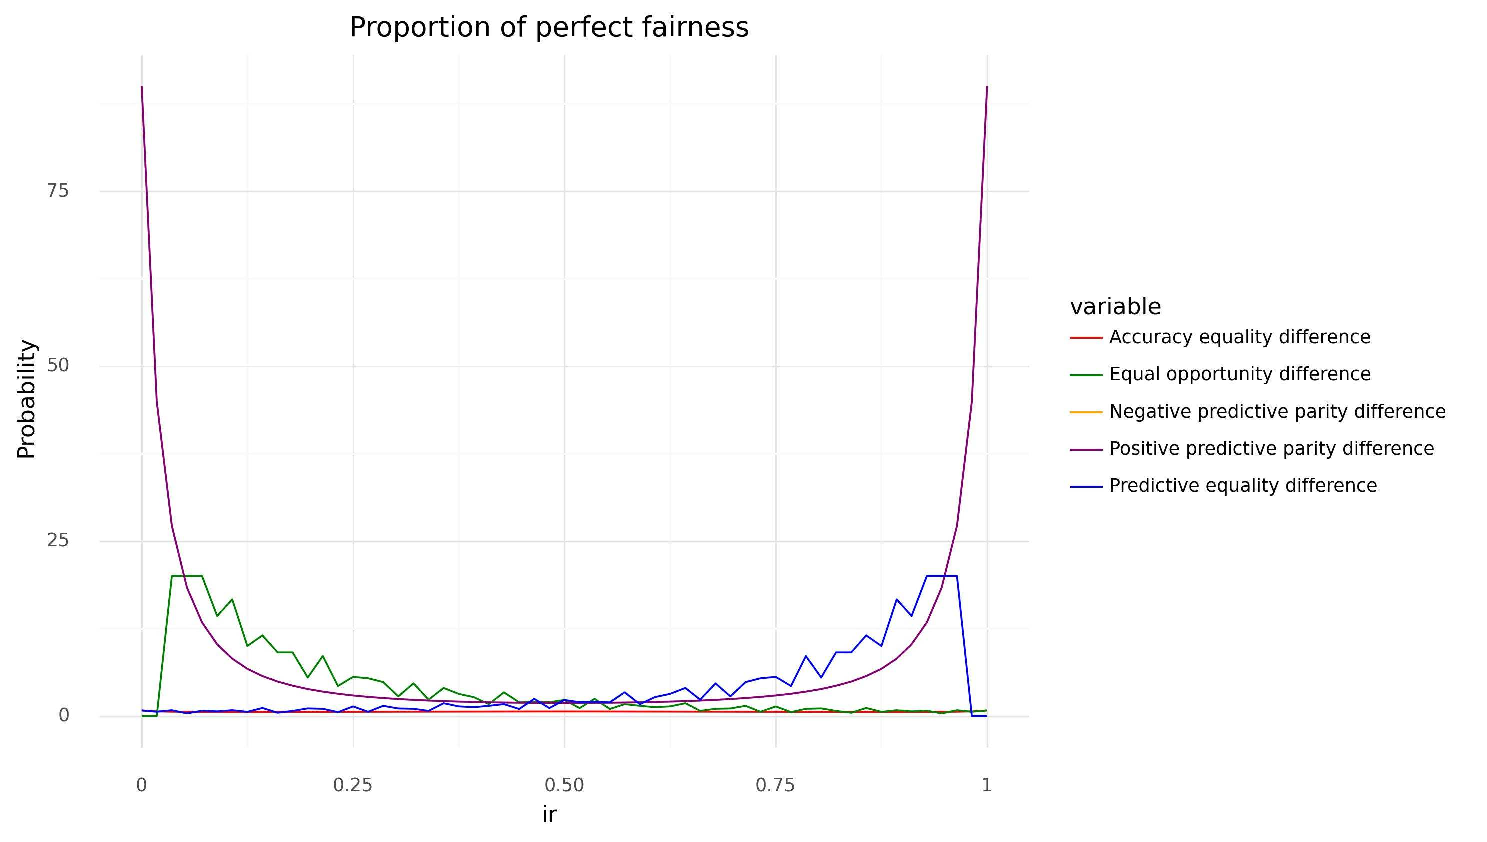
\includegraphics[width=0.9\textwidth]{PPF}
\caption{Proportion of Perfect Fairness Plot}\label{fig2}
\end{figure}

In contrast to the NPPD metric, the SP metric, as depicted in Figure ~\ref{fig3}, demonstrates a consistent level of perfect fairness for the [EP] Table ~\ref{tab2} property. However, it is important to also consider the [HP] property in conjunction with this. While the SP metric shows results that are equally probable to be fair regardless of the IR value, these probabilities barely exceed 0.05. This means that, despite an equal level of fairness, the overall probability of fairness is extremely low.

\begin{figure}[h]%
\centering
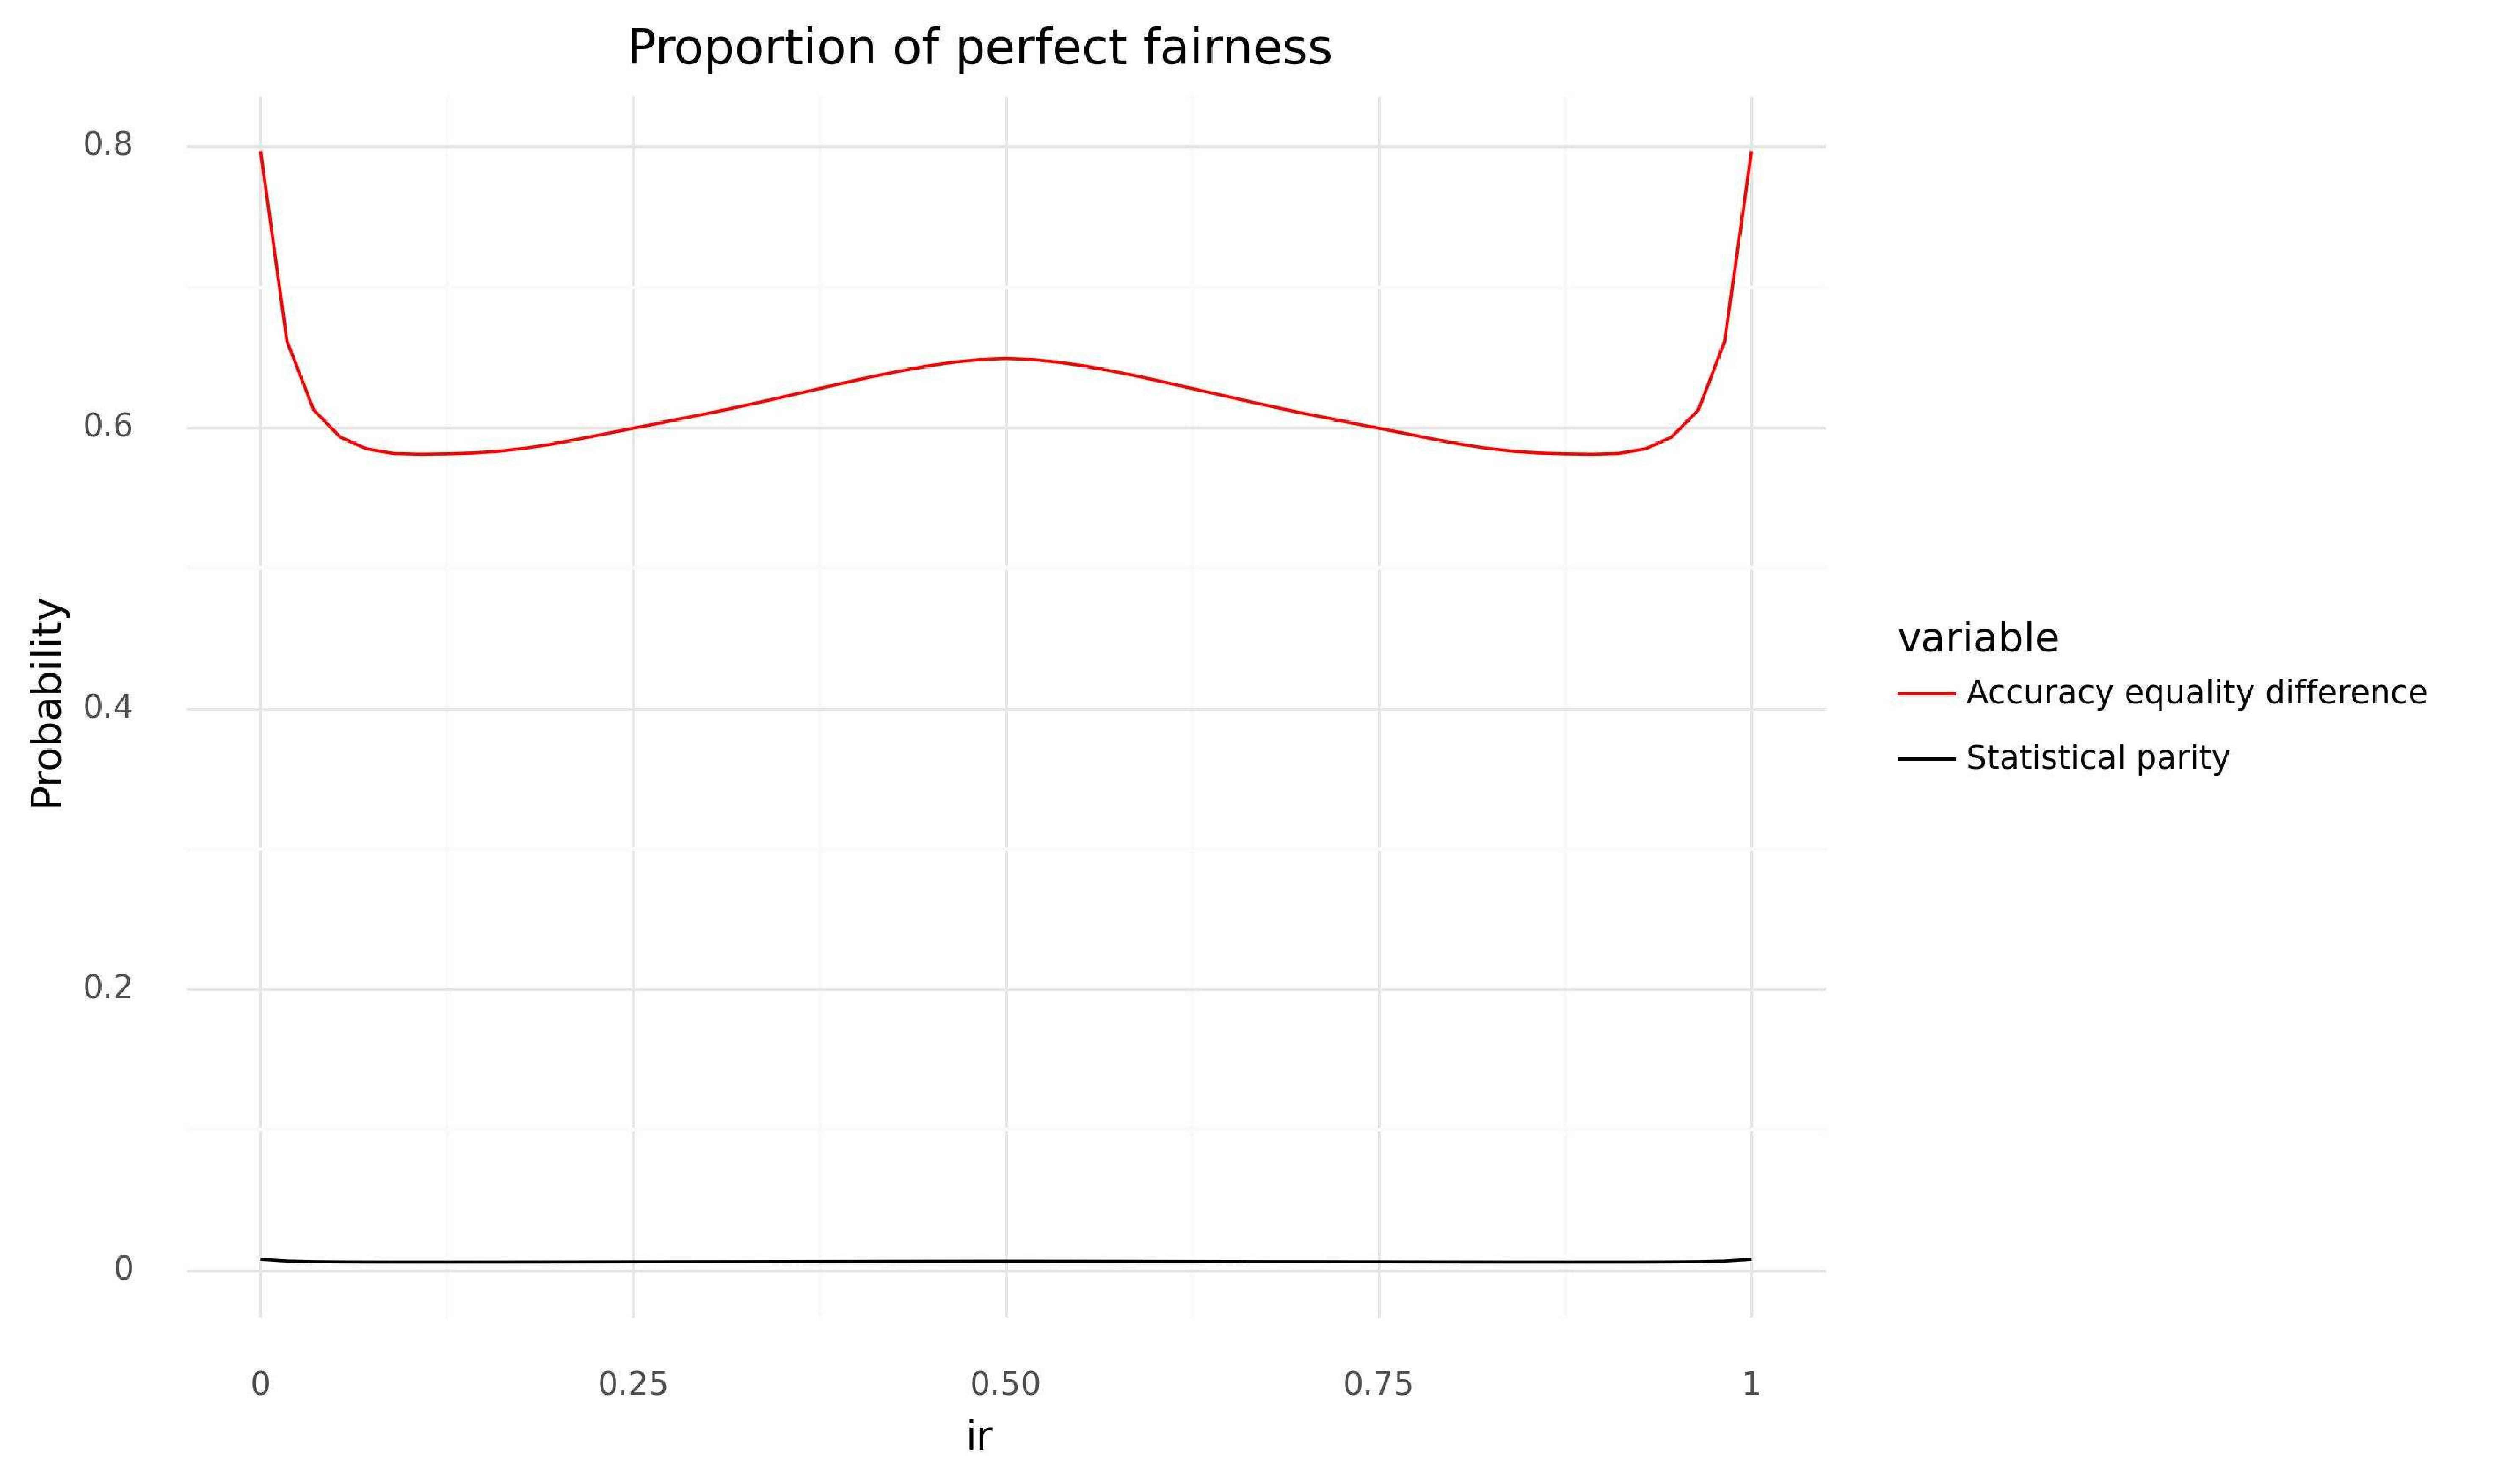
\includegraphics[width=0.9\textwidth]{PPF4}
\caption{Proportion of Perfect Fairness Plot (high resolution)}\label{fig3}
\end{figure}

\subsubsection{Proportion of Perfect Fairness}\label{subsubsec2}

Each metric behavior can be also observed on PPF plots in supplementary materials, some of them are presented as Figure ~\ref{fig2}, Figure ~\ref{fig3}. The results reveal that for the EOD, PED, PPPD, and NPPD measures, the highest probability of achieving fairness ($\approx$ 0.9) is only attained when the dataset is fully represented by one group. When the proportion of minority and majority groups is equal, the chances of achieving fairness are low (less than 5\%).

The probability of achieving fairness as determined by the AED measure is close to zero, with a maximum value of approximately 0.008. This result is consistent with the SP measure, which also approaches zero.

\section{Conclusions}\label{sec5}

Coming back to our initial question, different types of data bias can affect the performance of fairness measures in different ways.

For example, if the data is biased towards a certain group, such as a majority group, the performance of metrics like accuracy equality difference (AED) and statistical parity (SP) may be affected. If the majority group has a higher accuracy or proportion of positive outcomes compared to the minority group, then the AED and SP will be high, indicating a lack of fairness.

If the data is biased in terms of class imbalance, the performance of metrics like equal opportunity difference (EOD) and predictive equality difference (PED) may be affected. If the majority class has a higher true positive rate or false positive rate compared to the minority class, then the EOD and PED will be high, indicating a lack of fairness.

However, if the data is biased in terms of predictive values, the performance of metrics like positive predictive parity difference (PPPD) and negative predictive parity difference (NPPD) may be affected. If the majority group has a higher positive predictive value or negative predictive value compared to the minority group, then the PPPD and NPPD will be high, indicating a lack of fairness.

The conducted analysis has yielded novel findings, as it diverges from previous studies. Despite this progress, there remains plenty of unexplored concepts that could be utilized in future research.

\backmatter

\bmhead{Supplementary information}

The entire set of plots can be found in the online supplementary materials.

\begin{thebibliography}{9}

\bibitem{bib1} Simon Canton and Christian Haas. Fairness in machine learning: A survey. 2020.

\bibitem{bib2} Xu-ying Liu and Zhi-hua Zhou. The influence of class imbalance on cost-sensitive learning: An empirical study. In Sixth International Conference on Data Mining (ICDM’06), pages 970–974, 2006.

\bibitem{bib3} Anahideh, H., Nezami, N. and Asudeh, A. (2021) “On the choice of fairness: Finding representative fairness metrics for a given context,” arXiv [cs.LG]. Available at: http://arxiv.org/abs/2109.05697.

\bibitem{bib4} S. Mishra. Handling imbalanced data: Smote vs. random undersampling. International Research Journal of Engineering and Technology, 04:317–320, 2017.

\bibitem{bib5} Brzezinski, D. et al. (2018) “Visual-based analysis of classification measures a for class imbalanced problems,” Information Sciences, 462, pp. 242–261.

\bibitem{bib6} Mehrabi, N. et al. (2021) “A survey on bias and fairness in machine learning,” ACM computing surveys, 54(6), pp. 1–35.

\bibitem{bib7} Prati R. Batista, G. and M. Monard. A study of the behavior of several methods for balancing machine learning training data. ACM SIGKDD Explorations Newsletter 6, 1:20–29, 2004.

\end{thebibliography}

\bibliography{sn-bibliography}

\end{document}
